% homework/hw11/hw11.tex
% Year 7 - Homework Packet 11: 180 Degrees Apart.
%
% Maths 5.1 (A sum of 360) and 5.2 (Intersecting lines); Science 3.4 (Tides),
% 3.5 (Energy) and 3.6 (Changes in energy). The teacher asked (28 Oct 2026) for
% "questions that provide interplay between the subjects", so:
%   Part 1  Sections A-B. The maths, as language: the two steps, then reasons
%           after "because". Maths first, as always.
%   Part 2  Sections C-E. The three science lessons, in words.
%   Part 3  Section F. Where they meet. F1 is the title: the two tidal bulges
%           are on a straight line through the Earth, 180 degrees apart, and
%           the Earth turns 15 degrees an hour, so high tide comes every 12
%           hours -- and the extra 12 degrees a day is the deck's "about 50
%           minutes later". F2 is the Sun, the Earth and the Moon in a line
%           (180) or at right angles (90). F3 is a pizza whose angles are its
%           joules. F4 is a wind turbine and a fan: angles round a point, and
%           two energy changes that are each other backwards. F5 is the writing.
% Extra Homework 11 (homework/hw11x, How High Does It Bounce?) goes out with it.
%
% Nothing untaught:
%   * 5.1: 180 on a line, 360 round a point and in a quadrilateral, the two
%     steps (add, then subtract), "sum", opposite angles of a parallelogram,
%     full turns (the deck's chair: 2.5 x 360). 5.2: vertically opposite,
%     parallel and perpendicular, corresponding (F), alternate (Z), "give a
%     reason" = the fact after "because", no arrows = need more information.
%   * 3.4: the write notes (tide, tidal range, tidal force, earth tide), two
%     bulges and the near/far stretch, high to low 6 hours, high to high 12,
%     about 50 minutes later each day (24 h / 29), the Sun 390 times further
%     away with about half the Moon's tidal force, biggest tides at full and
%     new moon. The 6 m / 2 m ranges in F2 are the LineThemUp model's (in a
%     line / at right angles). Hanoi's 30 cm earth tide.
%   * 3.5: the five stores and three transfers (thermal on both lists), the
%     book's joules (2 000 J a floor of stairs, 200 J a metre run, 400 000 J
%     to boil 1 litre), which stores last. 3.6: event and process, energy-
%     change diagrams read as "to", charging a phone is electrical TO
%     chemical, the bouncing ball (sound and heat at the bounce), thermal
%     energy moves from hotter to colder (the freezer vote).
%   * The 12 degrees a day in F1(e): the Moon goes round in about 29 days,
%     360 / 29 = 12.4. The 1 degree every 4 minutes is 1 440 / 360.
%   * Nothing from 3.7 (useful and wasted energy, percentages, dissipated).
%   * No number is lifted from the Workbook or from the decks' practice.
%
% House style is shared: see homework/hw-style.tex. Method: the new-homework
% skill. Source is pure ASCII on purpose.
%
% Build:  pwsh .claude/skills/new-homework/scripts/build-hw.ps1 hw11 -French

\documentclass[12pt,a4paper]{article}

% -- Answer key switch -------------------------------------------------------
\newif\ifkey
\ifdefined\TEACHER\keytrue\else
  \keyfalse        % \keyfalse = student copy   |   \keytrue = teacher copy
\fi

% -- Language switch ---------------------------------------------------------
% The French copy (hw11-fr.pdf) is this file built with \FRENCH defined. See
% hw09/README.md for the scheme.
\newif\iffr
\ifdefined\FRENCH\frtrue\fi

% -- House style -------------------------------------------------------------
% homework/hw-style.tex
% Shared house style for every Year 7 homework packet. \input this from the
% packet file, right after \documentclass and the answer-key switch.
%
% Do not fork this file per packet. If a packet needs a different look, the
% question is whether every packet should have it.
%
% The choices here are deliberate and were arrived at by printing and looking:
%   * No solid dark banners. Every header is a light tint with a coloured spine
%     on the left, so colour reads clearly without flooding a school printer.
%   * No marks and no mark totals. These are practice, not exam papers.
%   * Lato at 12pt with open leading, plus mathastext so inline maths is Lato
%     too. Without mathastext every "-6 + 4" is Computer Modern serif and the
%     sheet looks half-typeset.
%   * Writing lines are spaced for Year 7 handwriting, not adult margin notes.
%   * Pages fill. \needspace is redefined below so a heading no longer drags
%     the page break up to itself, and every heading is glued to the box under
%     it. Packets built before 2026-09-30 were laid out under the old rules and
%     will reflow if rebuilt -- re-read every page if you rebuild one.
%
% Provides: \wlines \blank \tickbox \sep \qmk-free marks (none) \hwsection
% \qhead \expr, the workspace box, and the remember / wordhelp / activity /
% yourturn coloured boxes. Palette matches the lesson decks exactly.

% -- Packages ----------------------------------------------------------------
\usepackage[T1]{fontenc}
\usepackage[utf8]{inputenc}
\usepackage[default]{lato}
\usepackage[a4paper,top=1.7cm,bottom=1.7cm,left=2.0cm,right=2.0cm,headheight=15pt]{geometry}
\usepackage{amsmath,amssymb}
\usepackage{xcolor}
\usepackage[most]{tcolorbox}
\usepackage{enumitem}
\usepackage{tikz}
\usetikzlibrary{arrows.meta}
\usepackage{array}
\usepackage{tabularx}
\usepackage{fancyhdr}
\usepackage{multicol}
\usepackage{needspace}
\usepackage{graphicx}

% Make maths use Lato too. Without this, every "-6 + 4" on the page is set in
% Computer Modern serif and the sheet looks half-typeset. Must come last.
\usepackage[italic]{mathastext}

% -- \needspace, without the hole it used to leave ----------------------------
% needspace.sty writes "\vskip 0pt plus X \penalty-100" in front of every
% heading. A page that ends anywhere else is underfull with no stretch, so TeX
% scores it b=10000; a page that ends AT a heading gets that X of stretch and a
% finite badness, and wins. So any heading in roughly the bottom half of a page
% claimed the break, and the question under it moved over whole, leaving a hole
% the size of the question. \tracingpages showed it exactly (b=4531 at the
% heading, b=10000 at every later break) while building homework/q1rev, and it
% is where the half-empty pages in HW 1-8 came from.
% This keeps only the \penalty9999, which still refuses to put a heading in the
% last X of a page. Keeping a heading WITH the box under it is \nobreak's job
% now -- see \hwsection and \qhead below.
\makeatletter
\renewcommand{\needspace}[1]{\begingroup\setlength{\dimen@}{#1}%
  \vskip\dimen@\penalty9999\vskip-\dimen@\endgroup}
\makeatother

\linespread{1.06}\selectfont

% -- The Learner's Book palette (same hex values as the lesson decks) ---------
\definecolor{cbteal}{HTML}{0087A8}
\definecolor{cbpurple}{HTML}{5C2483}
\definecolor{cborange}{HTML}{C25E12}
\definecolor{cbgreen}{HTML}{4A8B23}
\definecolor{cbred}{HTML}{C8102E}
\definecolor{cbblue}{HTML}{1A5FA8}
\definecolor{rulegray}{HTML}{9AA5AD}

% -- Answer lines and blanks -------------------------------------------------
% \wlines{n} draws n ruled writing lines, spaced wide enough for Year 7
% handwriting rather than for an adult with a fine pen.
\makeatletter
\newcommand{\wlines}[1]{%
  \par\vspace{0.75em}%
  \@tempcnta=0\relax
  \@whilenum\@tempcnta<#1\do{%
    \hbox to \linewidth{\color{rulegray}\leaders\hrule height 0.5pt\hfill}%
    \vspace{1.5em}%
    \advance\@tempcnta by 1\relax}%
  \par\vspace{-0.8em}%
}
\makeatother

% \blank[width] is an inline gap to write a short answer in.
\newcommand{\blank}[1][2.6cm]{\underline{\hspace{#1}}}

% A boxed space for showing working.
\newtcolorbox{workspace}[1][3.4cm]{%
  colback=white, colframe=rulegray, boxrule=0.5pt, arc=5pt,
  height=#1, left=6pt, right=6pt, top=4pt, bottom=4pt,
  before skip=9pt, after skip=11pt}

% An empty tick box.
\newcommand{\tickbox}{\fbox{\rule{0pt}{1.15em}\rule{1.15em}{0pt}}}

% A middot separator.
\newcommand{\sep}{\,\textperiodcentered\,}

% -- Section and question headings -------------------------------------------
% Light tint plus a fat coloured spine on the left. No solid dark banner: the
% colour reads clearly but barely costs the printer anything.
% needspace keeps a heading out of the last few lines of a page. The \nobreak
% after it keeps it with whatever comes next: a remember or word-help box that
% does not fit takes its heading over with it, instead of leaving the heading
% alone at the foot of the page. (The old needspace did that by accident, and
% left a hole every time; see above.)
\newcommand{\hwsection}[2][cbteal]{%
  \needspace{8\baselineskip}%
  \par\vspace{13pt}%
  \noindent
  \begin{tcolorbox}[enhanced, nobeforeafter, width=\textwidth,
      colback=#1!7, colframe=#1!7, arc=5pt,
      borderline west={5pt}{0pt}{#1},
      left=14pt, right=10pt, top=7pt, bottom=7pt]
    {\large\bfseries\color{#1}#2}
  \end{tcolorbox}%
  \par\nobreak\vspace{9pt}}

% \qhead[colour]{A2}{Moving along the line} -- a question heading.
\newcommand{\qhead}[3][cbteal]{%
  \needspace{6\baselineskip}%
  \par\vspace{11pt}%
  \noindent{\large\bfseries\color{#1}#2}\quad{\large\bfseries #3}\par\nobreak\vspace{4pt}}

% -- Coloured boxes ----------------------------------------------------------
% Shared look: rounded, light fill, coloured rule, coloured title text on a
% pale title strip rather than a dark one.
% NOT breakable. A breakable box that cannot fit its first lines forces its own
% page break, and \nobreak cannot stop a forced break -- so the heading above
% it was left alone at the foot of the page (tested: it happens with \nobreak
% in place). Unbreakable, the page builder moves heading and box together.
% These boxes are a few lines each; none needs to split.
\tcbset{hwbox/.style={
  enhanced, arc=6pt, boxrule=1pt,
  left=11pt, right=11pt, top=8pt, bottom=8pt,
  fonttitle=\bfseries, attach boxed title to top left={xshift=12pt, yshift=-8pt},
  boxed title style={arc=4pt, boxrule=1pt, left=7pt, right=7pt, top=2pt, bottom=2pt},
  top=13pt}}

% Orange: things to remember. Matches the deck's "Write This Down".
\newtcolorbox{remember}[1][Remember from the lesson]{hwbox,
  colback=cborange!6, colframe=cborange, coltitle=cborange,
  colbacktitle=white, title={#1}}

% Blue: English help. The barrier in this class is the wording, not the maths.
\newtcolorbox{wordhelp}[1][Word help]{hwbox,
  colback=cbblue!6, colframe=cbblue, coltitle=cbblue,
  colbacktitle=white, title={#1}}

% Purple: an activity or instruction.
\newtcolorbox{activity}[1][How to do this homework]{hwbox,
  colback=cbpurple!6, colframe=cbpurple, coltitle=cbpurple,
  colbacktitle=white, title={#1}}

% Green: your turn / a friendly nudge.
\newtcolorbox{yourturn}[1][Your turn]{hwbox,
  colback=cbgreen!7, colframe=cbgreen, coltitle=cbgreen!75!black,
  colbacktitle=white, title={#1}}

% -- Shorthands --------------------------------------------------------------
\newcommand{\dC}{\,^{\circ}\mathrm{C}}          % use inside maths: $-8\dC$
\newcommand{\key}[1]{{\color{cborange}\textbf{#1}}}
\newcommand{\eng}[1]{{\color{cbblue}\textbf{#1}}}

\setlist[enumerate]{itemsep=8pt, topsep=5pt, leftmargin=*}
\setlist[itemize]{itemsep=4pt, topsep=4pt, leftmargin=*}
\renewcommand{\arraystretch}{1.45}

% -- An expression the student is asked to work from -------------------------
\newcommand{\expr}[1]{%
  \tcbox[on line, colback=cbgreen!10, colframe=cbgreen!55, boxrule=1pt, arc=4pt,
         left=9pt, right=9pt, top=4pt, bottom=4pt]{\large\bfseries $#1$}}

% -- Running head and foot ---------------------------------------------------
% The packet overrides \fancyhead[L] with its own title.
\pagestyle{fancy}
\fancyhf{}
\fancyhead[L]{\small\color{black!55}Year 7\sep Homework}
\fancyhead[R]{\small\color{black!55}Name: \blank[3.4cm]}
\fancyfoot[C]{\small\color{black!55}Page \thepage}
\renewcommand{\headrulewidth}{0pt}
\renewcommand{\headrule}{\vspace{2pt}\hbox to\headwidth{\color{cbteal!45}\leaders\hrule height 1.2pt\hfill}}


\usetikzlibrary{angles,quotes,calc}

% -- French support lines ----------------------------------------------------
% \fr{...}  a French line of its own, grey and italic, under the English.
% \frin{...} a French gloss in brackets, inline -- for table cells and labels.
% Both are EMPTY in the English copy, and both start with \unskip so the line
% break before them cannot leave a space that moves an English break.
\newcommand{\fr}[1]{\unskip\iffr\par\nobreak\vspace{1pt}\noindent{\small\itshape\color{black!60}#1}\par\fi}
\newcommand{\frin}[1]{\unskip\iffr\ {\small\itshape\color{black!60}(#1)}\fi}
\newcommand{\fq}[1]{\guillemotleft\,#1\,\guillemotright}

% -- Per-packet running head -------------------------------------------------
\iffr
  \fancyhead[L]{\small\color{black!55}Year 7\sep Homework 11\sep English /
    Fran\c{c}ais}
\else
  \fancyhead[L]{\small\color{black!55}Year 7\sep Homework 11}
\fi

% -- English size, French size -----------------------------------------------
% \frl{english}{french}: a box height or a number of writing lines that is
% bigger in the French copy.
\newcommand{\frl}[2]{\iffr#2\else#1\fi}

% -- Degrees, inside maths: $72\dg$ ------------------------------------------
\newcommand{\dg}{^{\circ}}

% -- A group of writing lines that will not be split -------------------------
\newcommand{\qlines}[1]{\par\nobreak
  \noindent\begin{minipage}{\linewidth}\wlines{#1}\end{minipage}\par}

% -- A box to write one letter or sign in ------------------------------------
\newcommand{\nbox}{\ \fbox{\rule{0pt}{1.05em}\rule{1.0em}{0pt}}\ }

% -- An answer blank on a line of its own, right-aligned ---------------------
\newcommand{\ansline}[1][4.4cm]{\par\nobreak\vspace{2pt}\hspace*{\fill}\blank[#1]\par}

% -- "Calculation: ____  Answer: ____" on a line of its own -------------------
% The calculation comes FIRST on the line: it is the thing to write first.
\newcommand{\calcans}[1][6.6cm]{\par\nobreak\vspace{\frl{3pt}{5pt}}\noindent\hspace*{1.6em}%
  \textbf{Calculation:} \blank[#1] \hfill \textbf{Answer:} \blank[3.0cm]\par}

% -- Columns -----------------------------------------------------------------
\newcolumntype{L}{>{\raggedright\arraybackslash}X}
% \leavevmode, so a cell that starts with a \color is not dropped a line.
\newcolumntype{C}[1]{>{\centering\arraybackslash\leavevmode}p{#1}}
\newcolumntype{P}[1]{>{\leavevmode\raggedright\arraybackslash}p{#1}}
\newcolumntype{W}[1]{>{\leavevmode\raggedright\bfseries\color{cbblue}}p{#1}}

% -- A table row tall enough to write in -------------------------------------
\newcommand{\tall}{\rule[-0.6em]{0pt}{1.9em}}

% -- Drawing styles ----------------------------------------------------------
\definecolor{sunfill}{HTML}{FDE58A}
\definecolor{sunrim}{HTML}{C99A06}
\definecolor{seafill}{HTML}{CFE6F5}
\definecolor{landfill}{HTML}{CDE3B4}
\definecolor{pizzafill}{HTML}{F6D58E}
\definecolor{crust}{HTML}{C98A3A}
\tikzset{
  % an angle arc with its label: \pic[ang, "$72\dg$"] {angle = R--O--P};
  ang/.style={draw=cborange, line width=0.8pt, angle radius=0.42cm,
    angle eccentricity=1.75, pic text options={font=\small}},
  % the same, for the letter the student finds
  let/.style={draw=cbteal, line width=0.8pt, angle radius=0.36cm,
    angle eccentricity=1.75, pic text options={font=\small\bfseries\itshape, text=cbteal}},
  rt/.style={draw=black!70, line width=0.7pt, angle radius=0.25cm},
  % parallel arrows on a line, drawn at a point
  par/.style={line width=1pt, -{Stealth[length=6pt, width=6pt]}},
  % an energy-change box, and its arrow
  ebx/.style={draw=cbgreen!70!black, line width=0.8pt, rounded corners=3pt,
    minimum width=2.9cm, minimum height=0.85cm, font=\small\bfseries},
  earr/.style={line width=1.1pt, -{Stealth[length=7pt, width=6pt]}, cbgreen!60!black},
}

% -- More room in the French copy --------------------------------------------
% The French copy carries a second line under every question, so it gets more
% room to write as well: wider writing lines, taller table rows, working
% boxes a third taller. The English copy is untouched by all of this.
\iffr
  \linespread{1.10}\selectfont
  \renewcommand{\tall}{\rule[-0.8em]{0pt}{2.4em}}
  \renewtcolorbox{workspace}[1][3.4cm]{%
    colback=white, colframe=rulegray, boxrule=0.5pt, arc=5pt,
    height={1.33\dimexpr #1\relax}, left=6pt, right=6pt, top=4pt, bottom=4pt,
    before skip=9pt, after skip=11pt}
  \makeatletter
  \renewcommand{\wlines}[1]{%
    \par\vspace{0.75em}%
    \@tempcnta=0\relax
    \@whilenum\@tempcnta<#1\do{%
      \hbox to \linewidth{\color{rulegray}\leaders\hrule height 0.5pt\hfill}%
      \vspace{1.9em}%
      \advance\@tempcnta by 1\relax}%
    \par\vspace{-0.8em}}
  \makeatother
\fi

\begin{document}

% ===========================================================================
% COVER BLOCK
% ===========================================================================
\thispagestyle{fancy}

\begin{tcolorbox}[enhanced, colback=cbpurple!7, colframe=cbpurple!7, arc=7pt,
                  borderline west={6pt}{0pt}{cbpurple},
                  left=18pt, right=14pt, top=10pt, bottom=10pt]
  {\color{cbpurple}\bfseries YEAR 7\sep MATHS UNIT 5\sep SCIENCE UNIT 3\sep
  HOMEWORK 11}\\[5pt]
  {\color{cbpurple}\Huge\bfseries 180\textdegree\ Apart}\\[7pt]
  {\color{black!70}Part 1: Maths --- 5.1 A sum of 360\textdegree\ and 5.2
  Intersecting lines}\\
  {\color{black!70}Part 2: Science --- 3.4 Tides, 3.5 Energy and 3.6 Changes in
  energy}\\
  {\color{black!70}Part 3: Maths and science together}
  \iffr\\[4pt]{\small\itshape\color{black!60}\`A 180\textdegree\ l'une de
  l'autre~: les angles (5.1 et 5.2)~; les mar\'ees et l'\'energie (3.4 \`a 3.6)~;
  les maths et les sciences ensemble}\fi
\end{tcolorbox}

\vspace{4pt}
\noindent
\begin{tabularx}{\textwidth}{@{}X X@{}}
  \textbf{Name:} \blank[5.6cm] & \textbf{Class:} \blank[5.6cm] \\
  \textbf{Date given:} \blank[4.6cm] &
  \textbf{Date due:} {\color{cbred}\bfseries Friday 6 November 2026} \\
\end{tabularx}

\vspace{2pt}
\begin{activity}
  \begin{itemize}[itemsep=3pt, topsep=0pt]
    \item \textbf{A--B:} maths. \ \textbf{C--E:} science. \ \textbf{F:} both
          together. \ \key{No calculator.} Write the \key{calculation} first, then
          the answer.
          \frin{A et B~: maths~; C \`a E~: sciences~; F~: les deux ensemble.
          Calculatrice interdite. \'Ecris d'abord le calcul, puis le r\'esultat.}
    \item \key{Give a reason} = write the angle fact after \key{because}:
          \emph{``$a = 40\dg$ because they are vertically opposite angles.''}
          \frin{Donne une raison (\eng{give a reason})~: \'ecris la propri\'et\'e
          apr\`es \eng{because} (parce que).}
    \item Answer in \key{full sentences} when it says so. \emph{``Kinetic''} is not
          a sentence. \emph{``The bike has kinetic energy because it is moving''}
          is.
          \frin{R\'eponds par des phrases compl\`etes, \textbf{en anglais}, quand on
          te le demande.}
  \end{itemize}
\end{activity}

% ===========================================================================
% SECTION A -- MATHS 5.1: A SUM OF 360
% ===========================================================================
\hwsection{Section A \textperiodcentered\ Maths 5.1 --- A Sum of 360\textdegree}

% -- A1 ---------------------------------------------------------------------
% The two steps on six diagrams, drawn accurately. (a) is worked. (b) has one
% known angle, so step 1 is just that angle. (c)-(d) are round a point, (e) is
% a quadrilateral, (f) a parallelogram (opposite angles equal, then 360).
\qhead{A1}{Find the missing angle: two steps}

\begin{remember}[Two steps, from the lesson]
  \textbf{1.} \key{Add} the angles you know. \quad \textbf{2.} \key{Subtract} the
  total from \key{180\textdegree} (a straight line) or \key{360\textdegree}
  (around a point, or in a quadrilateral). \\
  In a \key{parallelogram}, opposite angles are \key{equal}.
  \fr{1. Additionne les angles que tu connais. 2. Soustrais le total de 180\textdegree\
  (une ligne droite) ou de 360\textdegree\ (autour d'un point, ou dans un
  quadrilat\`ere). Dans un parall\'elogramme, les angles oppos\'es sont \'egaux.}
\end{remember}

% \atwo{letter}{the drawing}{the working lines}
\newcommand{\atwo}[3]{%
  \begin{minipage}[t]{0.315\textwidth}
    \textbf{(#1)}\par\vspace{2pt}
    \parbox[c][\frl{3.2cm}{3.7cm}][c]{\linewidth}{\centering #2}\par
    \vspace{4pt}
    {\renewcommand{\arraystretch}{\frl{1.55}{1.8}}%
    \begin{tabular}{@{}l@{\ }l@{}}#3\end{tabular}}
  \end{minipage}}
% the empty working, for every diagram but (a)
\newcommand{\aworkB}[1]{%
  \textbf{1.} & \blank[3.3cm] \\
  \textbf{2.} & \blank[3.3cm] \\
  \textbf{#1} $=$ & \blank[2.2cm] \\}

% The instruction and the first row are one block, so the instruction is
% never left at the foot of a page without its diagrams (French copy).
\noindent\begin{minipage}{\textwidth}
\noindent The diagrams are drawn accurately. Find each letter. (a) is done for you.
\fr{Trouve chaque lettre. Le (a) est fait pour toi.}

\vspace{6pt}
\noindent
\atwo{a}{%
  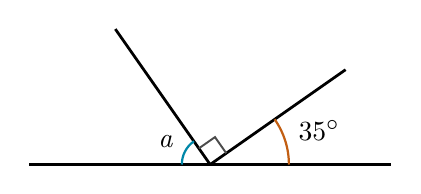
\begin{tikzpicture}[line width=1pt]
    \coordinate (O) at (0,0); \coordinate (L) at (-2.3,0); \coordinate (R) at (2.3,0);
    \coordinate (P) at (35:2.1); \coordinate (Q) at (125:2.1);
    \draw (L) -- (R); \draw (O) -- (P); \draw (O) -- (Q);
    \pic[ang, angle radius=1.0cm, angle eccentricity=1.45, "$35\dg$"] {angle = R--O--P};
    \pic[rt] {right angle = P--O--Q};
    \pic[let, "$a$"] {angle = Q--O--L};
  \end{tikzpicture}}{%
  \textbf{1.} & {\color{cbteal}$35\dg + 90\dg = 125\dg$} \\
  \textbf{2.} & {\color{cbteal}$180\dg - 125\dg = 55\dg$} \\
  \textbf{a} $=$ & {\color{cbteal}$55\dg$} \\}\hfill
\atwo{b}{%
  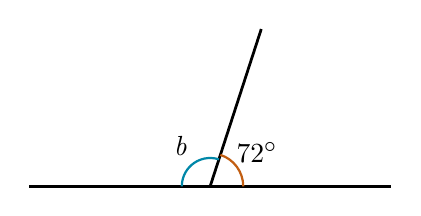
\begin{tikzpicture}[line width=1pt]
    \coordinate (O) at (0,0); \coordinate (L) at (-2.3,0); \coordinate (R) at (2.3,0);
    \coordinate (P) at (72:2.1);
    \draw (L) -- (R); \draw (O) -- (P);
    \pic[ang, "$72\dg$"] {angle = R--O--P};
    \pic[let, "$b$"] {angle = P--O--L};
  \end{tikzpicture}}{\aworkB{b}}\hfill
\atwo{c}{%
  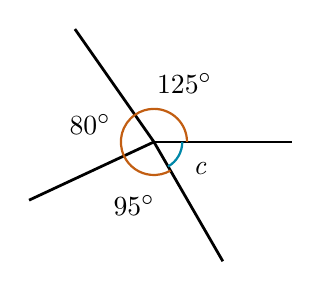
\begin{tikzpicture}[line width=1pt]
    \coordinate (O) at (0,0); \coordinate (R) at (0:1.75);
    \coordinate (P) at (125:1.75); \coordinate (Q) at (205:1.75);
    \coordinate (S) at (300:1.75);
    \draw (O) -- (R); \draw (O) -- (P); \draw (O) -- (Q); \draw (O) -- (S);
    \pic[ang, "$125\dg$", angle eccentricity=2.0] {angle = R--O--P};
    \pic[ang, "$80\dg$", angle eccentricity=2.0] {angle = P--O--Q};
    \pic[ang, "$95\dg$", angle eccentricity=2.0] {angle = Q--O--S};
    \pic[let, "$c$", angle eccentricity=1.9] {angle = S--O--R};
  \end{tikzpicture}}{\aworkB{c}}
\end{minipage}

\vspace{10pt}
\noindent
\atwo{d}{%
  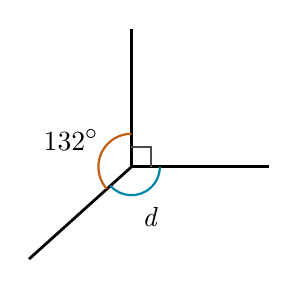
\begin{tikzpicture}[line width=1pt]
    \coordinate (O) at (0,0); \coordinate (R) at (0:1.75);
    \coordinate (P) at (90:1.75); \coordinate (Q) at (222:1.75);
    \draw (O) -- (R); \draw (O) -- (P); \draw (O) -- (Q);
    \pic[rt] {right angle = R--O--P};
    \pic[ang, "$132\dg$", angle eccentricity=2.0] {angle = P--O--Q};
    \pic[let, "$d$", angle eccentricity=1.9] {angle = Q--O--R};
  \end{tikzpicture}}{\aworkB{d}}\hfill
\atwo{e}{%
  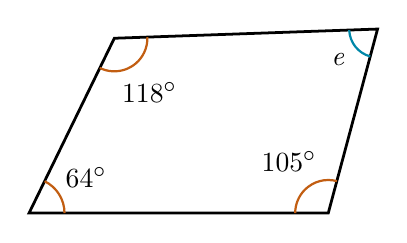
\begin{tikzpicture}[line width=1pt, scale=0.95]
    \coordinate (A) at (0,0); \coordinate (B) at (4,0);
    \coordinate (C) at (4.659,2.460); \coordinate (D) at (1.140,2.337);
    \draw (A) -- (B) -- (C) -- (D) -- cycle;
    \pic[ang, "$64\dg$", angle radius=0.45cm, angle eccentricity=1.9] {angle = B--A--D};
    \pic[ang, "$105\dg$", angle eccentricity=1.95] {angle = C--B--A};
    \pic[let, "$e$"] {angle = D--C--B};
    \pic[ang, "$118\dg$", angle eccentricity=1.95] {angle = A--D--C};
  \end{tikzpicture}}{\aworkB{e}}\hfill
\atwo{f}{%
  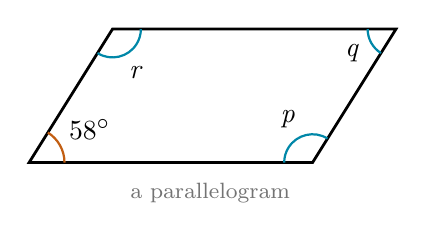
\begin{tikzpicture}[line width=1pt, scale=1.0]
    \coordinate (A) at (0,0); \coordinate (B) at (3.6,0);
    \coordinate (C) at (4.660,1.696); \coordinate (D) at (1.060,1.696);
    \draw (A) -- (B) -- (C) -- (D) -- cycle;
    \pic[ang, "$58\dg$", angle radius=0.45cm, angle eccentricity=1.95] {angle = B--A--D};
    \pic[let, "$p$"] {angle = C--B--A};
    \pic[let, "$q$"] {angle = D--C--B};
    \pic[let, "$r$"] {angle = A--D--C};
    \node[font=\footnotesize, text=black!55, anchor=north] at (2.3,-0.12)
      {a parallelogram};
  \end{tikzpicture}}{%
  \textbf{q} $=$ & \blank[2.6cm] \\
  \textbf{1.} & \blank[3.3cm] \\
  \textbf{p} $=$ \textbf{r} $=$ & \blank[1.9cm] \\}

% -- A2 ---------------------------------------------------------------------
% THE LANGUAGE QUESTION. Every item is decided by its English. (a) is the
% deck's vote (57 + 121 = 178) with new numbers: 63 + 116 = 179, which looks
% straight and is not. "The sum of two angles is 180" is a straight line with
% no picture; "the other three are equal" is a division after the
% subtraction; "how many full turns" is a division by 360.
\qhead{A2}{From English to a calculation}

\begin{wordhelp}[Word help --- the words in angle questions]
  \renewcommand{\arraystretch}{1.25}%
  \begin{tabularx}{\linewidth}{@{}W{2.3cm}L W{3.3cm}L@{}}
    sum & the total when you add \frin{la somme} & work out & find, and show the
      calculation \frin{calcule} \\
    equal & the same size \frin{\'egaux} & a full turn & 360\textdegree \frin{un tour
      complet} \\
  \end{tabularx}
\end{wordhelp}

\vspace{2pt}
\noindent Write the \textbf{calculation first}. Then write the answer.
\fr{\'Ecris d'abord le calcul, puis le r\'esultat.}

\begin{enumerate}[label=(\alph*), itemsep=6pt]
  \item Two angles are $63\dg$ and $116\dg$. Mr Bowen says they make a
        \textbf{straight line}. Is he right?
        \fr{Deux angles font $63\dg$ et $116\dg$. Mr Bowen dit qu'ensemble ils font une
        ligne droite. A-t-il raison~?}
        \calcans
  \item The sum of two angles is $180\dg$. One of them is $64\dg$. Work out the
        other one.
        \fr{La somme de deux angles est $180\dg$. L'un des deux fait $64\dg$. Calcule
        l'autre.}
        \calcans
  \item Three angles of a quadrilateral are $90\dg$, $90\dg$ and $47\dg$. Calculate
        the fourth angle.
        \fr{Trois angles d'un quadrilat\`ere font $90\dg$, $90\dg$ et $47\dg$. Calcule le
        quatri\`eme angle.}
        \calcans
  \item One angle of a quadrilateral is $120\dg$. The other three angles are
        equal. Work out the size of each one.
        \fr{Un angle d'un quadrilat\`ere fait $120\dg$. Les trois autres sont \'egaux.
        Calcule la taille de chacun.}
        \calcans
  \item Mr Bowen spins round on his chair. He turns through $1080\dg$. How many
        full turns is that?
        \fr{Mr Bowen tourne sur sa chaise. Il tourne de $1080\dg$. Combien de tours
        complets (\eng{full turns}) cela fait-il~?}
        \calcans
\end{enumerate}

% -- A3 ---------------------------------------------------------------------
% Calculation -> English. A minipage: the rules and the expression must stay
% together.
\qhead{A3}{Now you write the question}

\noindent\begin{minipage}{\textwidth}
\noindent Write a word problem for \quad
\expr{360\dg - 70\dg - 110\dg - 95\dg = 85\dg}
\fr{Invente, en anglais, un probl\`eme (\eng{word problem}) qui correspond \`a ce
calcul.}

\begin{yourturn}[Your word problem must have: tick each one]
  \renewcommand{\arraystretch}{1.35}%
  \begin{tabularx}{\linewidth}{@{}p{0.75cm}L p{0.75cm}L p{0.75cm}L@{}}
    \tickbox & a real thing (a garden, a kite \ldots) & \tickbox & the word
      \textbf{quadrilateral} & \tickbox & three angles \\
    \tickbox & full sentences & \tickbox & a question at the end & \tickbox & the
      answer 85\textdegree \\
  \end{tabularx}
  \fr{Une vraie chose (un jardin, un cerf-volant\ldots), le mot \eng{quadrilateral},
  trois angles, des phrases compl\`etes, une question \`a la fin, et la r\'eponse
  85\textdegree. \textbf{\'Ecris ton probl\`eme en anglais.}}
\end{yourturn}
\wlines{\frl{4}{5}}
\end{minipage}

% ===========================================================================
% SECTION B -- MATHS 5.2: INTERSECTING LINES
% ===========================================================================
\hwsection{Section B \textperiodcentered\ Maths 5.2 --- Intersecting Lines}

% -- B1 ---------------------------------------------------------------------
% One X, one F, one Z, each answer with its reason; then the deck's "which
% statement is correct?" with new numbers: no arrows, so C.
\qhead{B1}{Find the angle. Give a reason.}

\begin{wordhelp}[The four reasons --- copy the one you need after \textbf{because}]
  \renewcommand{\arraystretch}{1.2}%
  \begin{tabularx}{\linewidth}{@{}p{9.2cm}L@{}}
    \textbf{X:} vertically opposite angles are equal &
    \textbf{F:} corresponding angles are equal \\
    \textbf{line:} angles on a straight line add up to 180\textdegree &
    \textbf{Z:} alternate angles are equal \\
  \end{tabularx}
  \par\vspace{3pt}\noindent\textbf{Example:} \ {\color{cbteal}$a = 137\dg$ because
  vertically opposite angles are equal.}
  \fr{Les quatre raisons, \`a recopier en anglais apr\`es \eng{because}~: angles
  oppos\'es par le sommet~; angles sur une ligne droite~; angles correspondants~;
  angles alternes-internes.}
\end{wordhelp}

\noindent\begin{minipage}{\textwidth}
\noindent Arrows ($>$) on two lines mean they are \textbf{parallel}. Find each
letter, and give a reason.
\fr{Des fl\`eches ($>$) sur deux droites veulent dire qu'elles sont parall\`eles.
Trouve chaque lettre et donne une raison (l'exemple est dans la bo\^ite).}

\vspace{6pt}
\noindent
\begin{minipage}[b]{0.30\textwidth}\centering
  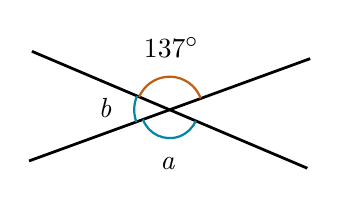
\begin{tikzpicture}[line width=1pt]
    \coordinate (O) at (0,0);
    \coordinate (A1) at (20:1.9); \coordinate (A2) at (200:1.9);
    \coordinate (B1) at (157:1.9); \coordinate (B2) at (337:1.9);
    \draw (A2) -- (A1); \draw (B2) -- (B1);
    \pic[ang, "$137\dg$", angle eccentricity=1.9] {angle = A1--O--B1};
    \pic[let, "$a$", angle eccentricity=1.9] {angle = A2--O--B2};
    \pic[let, "$b$", angle radius=0.45cm, angle eccentricity=1.8] {angle = B1--O--A2};
  \end{tikzpicture}\par\vspace{2pt}\textbf{(i)} two lines cross
\end{minipage}\hfill
\begin{minipage}[b]{0.33\textwidth}\centering
  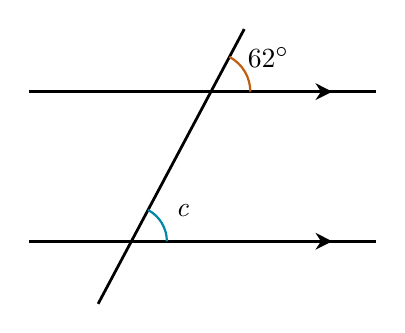
\begin{tikzpicture}[line width=1pt]
    \draw (0,0) -- (4.4,0); \draw (0,1.9) -- (4.4,1.9);
    \draw[par] (3.6,0) -- (3.85,0); \draw[par] (3.6,1.9) -- (3.85,1.9);
    \coordinate (B) at (1.3,0); \coordinate (T) at (2.310,1.9);
    \coordinate (TR) at (4.4,1.9); \coordinate (TU) at (2.733,2.695);
    \coordinate (BR) at (4.4,0);
    \draw (0.877,-0.795) -- (TU);
    \pic[ang, "$62\dg$", angle radius=0.5cm, angle eccentricity=1.7] {angle = TR--T--TU};
    \pic[let, "$c$", angle radius=0.45cm, angle eccentricity=1.7] {angle = BR--B--T};
  \end{tikzpicture}\par\vspace{2pt}\textbf{(ii)} parallel lines
\end{minipage}\hfill
\begin{minipage}[b]{0.33\textwidth}\centering
  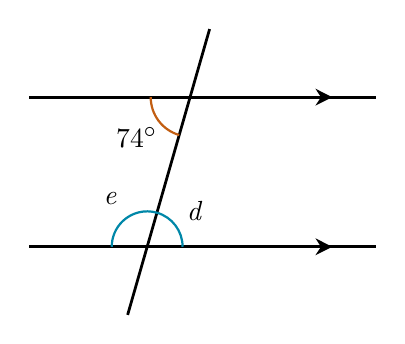
\begin{tikzpicture}[line width=1pt]
    \draw (0,0) -- (4.4,0); \draw (0,1.9) -- (4.4,1.9);
    \draw[par] (3.6,0) -- (3.85,0); \draw[par] (3.6,1.9) -- (3.85,1.9);
    \coordinate (B) at (1.5,0); \coordinate (T) at (2.045,1.9);
    \coordinate (TL) at (0,1.9); \coordinate (BR) at (4.4,0); \coordinate (BL) at (0,0);
    \draw (1.252,-0.865) -- (2.293,2.765);
    \pic[ang, "$74\dg$", angle radius=0.5cm, angle eccentricity=1.7] {angle = TL--T--B};
    \pic[let, "$d$", angle radius=0.45cm, angle eccentricity=1.7] {angle = BR--B--T};
    \pic[let, "$e$", angle radius=0.45cm, angle eccentricity=1.7] {angle = T--B--BL};
  \end{tikzpicture}\par\vspace{2pt}\textbf{(iii)} parallel lines
\end{minipage}
\end{minipage}

% The answer table is its own block, so the diagrams can end one page and the
% table start the next. A tabular never splits by itself.
\vspace{8pt}
\noindent\begin{minipage}{\textwidth}
{\renewcommand{\arraystretch}{\frl{1.6}{2.0}}%
\noindent\begin{tabular}{@{}l@{\ }l@{\ \ }l@{}}
  $b =$ & \blank[1.5cm] & because \blank[10.6cm] \\
  $c =$ & \blank[1.5cm] & because \blank[10.6cm] \\
  $d =$ & \blank[1.5cm] & because \blank[10.6cm] \\
  $e =$ & \blank[1.5cm] & because \blank[10.6cm] \\
\end{tabular}}
\end{minipage}

\vspace{10pt}
\noindent\begin{minipage}{\textwidth}
\noindent\begin{minipage}[c]{0.36\textwidth}\centering
  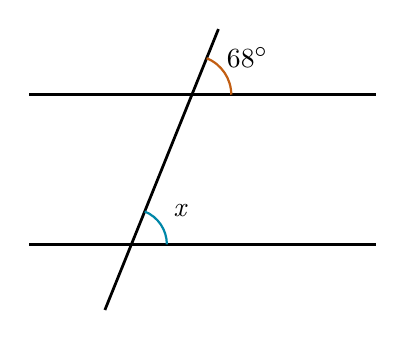
\begin{tikzpicture}[line width=1pt]
    \draw (0,0) -- (4.4,0); \draw (0,1.9) -- (4.4,1.9);
    \coordinate (B) at (1.3,0); \coordinate (T) at (2.068,1.9);
    \coordinate (TR) at (4.4,1.9); \coordinate (TU) at (2.405,2.734);
    \coordinate (BR) at (4.4,0);
    \draw (0.963,-0.834) -- (TU);
    \pic[ang, "$68\dg$", angle radius=0.5cm, angle eccentricity=1.7] {angle = TR--T--TU};
    \pic[let, "$x$", angle radius=0.45cm, angle eccentricity=1.7] {angle = BR--B--T};
  \end{tikzpicture}
\end{minipage}\hfill
\begin{minipage}[c]{0.61\textwidth}\raggedright
  \textbf{(iv)} Which statement is correct: \textbf{A}, \textbf{B} or \textbf{C}?
  \fr{(iv) Quelle phrase est correcte~: A, B ou C~?}
  \vspace{3pt}
  {\renewcommand{\arraystretch}{1.25}%
  \begin{tabular}{@{}l l@{}}
    \textbf{A} & $x = 68\dg$ \\
    \textbf{B} & $x = 112\dg$ \\
    \textbf{C} & You need more information. \frin{il faut plus d'informations} \\
  \end{tabular}}

  \vspace{4pt}
  \textbf{Answer:} \blank[1.2cm] \ \ because \blank[5.6cm]
  \par\vspace{10pt}\blank[\linewidth]
\end{minipage}
\end{minipage}

% -- B2 ---------------------------------------------------------------------
% One diagram, eight angles. Only (d) is right. (a) and (b) have the right
% angle and the wrong NAME; (c) has the wrong angle. See the key.
\qhead{B2}{Mr Bowen's homework}

\noindent\begin{minipage}{\textwidth}
\noindent\begin{minipage}[c]{0.38\textwidth}\centering
  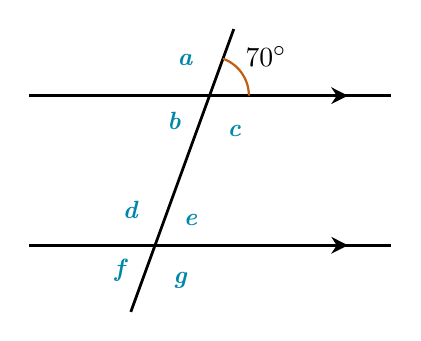
\begin{tikzpicture}[line width=1pt]
    \draw (0,0) -- (4.6,0); \draw (0,1.9) -- (4.6,1.9);
    \draw[par] (3.8,0) -- (4.05,0); \draw[par] (3.8,1.9) -- (4.05,1.9);
    \coordinate (B) at (1.6,0); \coordinate (T) at (2.292,1.9);
    \coordinate (TR) at (4.6,1.9); \coordinate (TU) at (2.600,2.746);
    \draw (1.292,-0.846) -- (TU);
    \pic[ang, "$70\dg$", angle radius=0.5cm, angle eccentricity=1.75] {angle = TR--T--TU};
    \foreach \p/\l in {125/a, 215/b, 305/c}
      \node[font=\small\bfseries\itshape, text=cbteal] at ($(T)+(\p:0.55)$) {\l};
    \foreach \p/\l in {125/d, 35/e, 215/f, 305/g}
      \node[font=\small\bfseries\itshape, text=cbteal] at ($(B)+(\p:0.55)$) {\l};
  \end{tikzpicture}
\end{minipage}\hfill
\begin{minipage}[c]{0.59\textwidth}\raggedright
  Only \textbf{one} of Mr Bowen's sentences is completely right. Circle
  \textbf{right} or \textbf{wrong}. If it is wrong, write the correct sentence.
  \fr{Une seule phrase de Mr Bowen est enti\`erement juste. Entoure \eng{right}
  (juste) ou \eng{wrong} (faux). Si elle est fausse, \'ecris la bonne phrase, en
  anglais.}
\end{minipage}
\end{minipage}

% Each sentence and its line are one unit, so the four can split across a page
% but a sentence never leaves its line behind.
\vspace{6pt}
\newcommand{\bthree}[2]{%
  \par\noindent\begin{minipage}{\textwidth}
  \noindent\textbf{(#1)} \ \emph{#2} \hfill right \ \sep\ wrong
  \par\vspace{\frl{12pt}{16pt}}\noindent\hspace*{1.6em}\blank[\dimexpr\linewidth-1.6em\relax]
  \end{minipage}\par\vspace{\frl{8pt}{10pt}}}
\bthree{a}{$b = 70\dg$ because they are corresponding angles.}
\bthree{b}{$e = 70\dg$ because they are alternate angles.}
\bthree{c}{$a = 70\dg$ because vertically opposite angles are equal.}
\bthree{d}{$d = 110\dg$ because $d$ and $c$ are alternate angles.}

% ===========================================================================
% SECTION C -- SCIENCE 3.4: TIDES
% ===========================================================================
\hwsection[cbgreen]{Section C \textperiodcentered\ Science 3.4 --- Tides}

% -- C1 ---------------------------------------------------------------------
% A day at a harbour, new numbers. (d) is the deck's "the same time
% tomorrow?". The book's Question 6 (average depth and range, not 7.0 m) is
% Extra Homework 11's X3, so it is not repeated here.
\qhead[cbgreen]{C1}{A day at the harbour}

\noindent\begin{minipage}{\textwidth}
Mr Bowen writes down the tides at his harbour for one day.
\fr{Mr Bowen note les mar\'ees de son port pendant une journ\'ee.}

\vspace{4pt}
{\centering
\renewcommand{\arraystretch}{\frl{1.3}{1.45}}%
\begin{tabular}{|l|*{4}{C{2.3cm}|}}
  \hline
  \textbf{Time} & 3 a.m. & 9 a.m. & 3 p.m. & 9 p.m. \\ \hline
  \textbf{Tide} & high tide & low tide & high tide & low tide \\ \hline
  \textbf{Depth} & 5.7 m & 1.3 m & 5.7 m & 1.3 m \\ \hline
\end{tabular}\par}
\end{minipage}

\vspace{6pt}
\begin{enumerate}[label=(\alph*), itemsep=\frl{5pt}{7pt}]
  \item How many high tides are there in one day? \hfill \blank[2.4cm]
        \fr{Combien y a-t-il de mar\'ees hautes en un jour~?}
  \item How many hours is it from high tide to low tide? \hfill \blank[2.4cm]
        \fr{Combien d'heures y a-t-il entre la mar\'ee haute et la mar\'ee basse~?}
  \item Work out the \textbf{tidal range}. \;
        {\small\color{cbblue}(\textbf{tidal range}: the difference in depth between
        high tide and low tide)}
        \fr{Calcule le marnage (\eng{tidal range}).}
        \calcans
  \item \begin{minipage}[t]{\linewidth}
        Tomorrow, will the first high tide be at 3 a.m. again? Answer in a full
        sentence. \; Start: \eng{``No, because the Moon \ldots''}
        \fr{Demain, la premi\`ere mar\'ee haute sera-t-elle encore \`a 3 h du matin
        (\eng{3 a.m.})~? R\'eponds par une phrase compl\`ete, en anglais.}
        \wlines{\frl{2}{3}}
        \end{minipage}
\end{enumerate}

% -- C2 ---------------------------------------------------------------------
% The deck's Draw This (page 99), to read instead of copy. A and C are the
% bulges (high tide); B and D are low. (b) is the far-side bulge: the deck's
% three students, 3 steps, 2 steps, 1 step.
\qhead[cbgreen]{C2}{Two high tides at the same time}

\noindent\begin{minipage}{\textwidth}
\noindent\begin{minipage}[c]{0.56\textwidth}\centering
  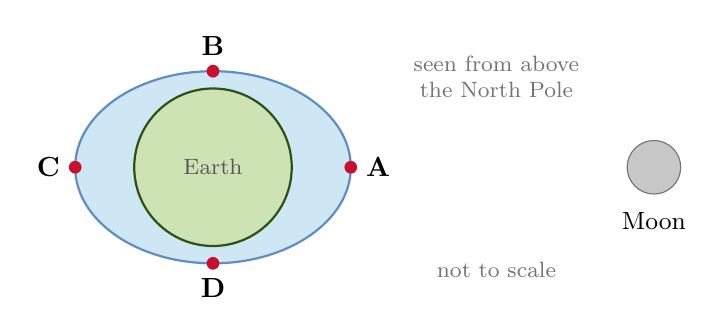
\begin{tikzpicture}
    \fill[seafill] (0,0) ellipse (1.75 and 1.22);
    \draw[cbblue!70, line width=0.8pt] (0,0) ellipse (1.75 and 1.22);
    \fill[landfill] (0,0) circle (1.0);
    \draw[cbgreen!60!black, line width=0.8pt] (0,0) circle (1.0);
    \node[font=\footnotesize, text=black!65] at (0,0) {Earth};
    \fill[black!22] (5.6,0) circle (0.34); \draw[black!55] (5.6,0) circle (0.34);
    \node[below=3pt, font=\small] at (5.6,-0.34) {Moon};
    \foreach \x/\y/\l/\pos in {1.75/0/A/right, 0/1.22/B/above, -1.75/0/C/left, 0/-1.22/D/below}
      {\fill[cbred] (\x,\y) circle (2.3pt); \node[\pos=2pt, font=\bfseries] at (\x,\y) {\l};}
    \node[font=\footnotesize, text=black!55, align=center] at (3.6,1.15)
      {seen from above\\the North Pole};
    \node[font=\footnotesize, text=black!55] at (3.6,-1.3) {not to scale};
  \end{tikzpicture}
\end{minipage}\hfill
\begin{minipage}[c]{0.41\textwidth}\raggedright
  \textbf{(a)} Is each place at \textbf{high tide} or \textbf{low tide}? Write
  \textbf{H} or \textbf{L}.
  \fr{(a) Chaque endroit est-il \`a mar\'ee haute (H) ou \`a mar\'ee basse (L)~?}

  \vspace{6pt}
  \textbf{A} \nbox \quad \textbf{B} \nbox \quad \textbf{C} \nbox \quad \textbf{D} \nbox
\end{minipage}

\vspace{8pt}
\noindent\textbf{(b)} The Moon is on the right. Why is there a high tide at
\textbf{C}, on the far side? \; Start: \eng{``The near side is pulled the most. The
far side \ldots''}
\fr{(b) La Lune est \`a droite. Pourquoi y a-t-il une mar\'ee haute en C, du c\^ot\'e
oppos\'e~? R\'eponds en anglais.}
\wlines{\frl{2}{3}}
\end{minipage}

% -- C3 ---------------------------------------------------------------------
% (a) is the deck's vote: the Sun pulls harder but stretches less (390 times
% further away). (b) is the earth tide's reveal.
\qhead[cbgreen]{C3}{The Sun, and the land}

\noindent\begin{minipage}{\textwidth}
\textbf{(a)} The Sun's gravity is \textbf{stronger} than the Moon's. Why does the
Moon make \textbf{bigger} tides? \; Start: \eng{``The Sun is much further away,
so \ldots''}
\fr{(a) La gravit\'e du Soleil est plus forte que celle de la Lune. Pourquoi la Lune
fait-elle de plus grandes mar\'ees~? R\'eponds en anglais.}
\wlines{\frl{2}{3}}
\end{minipage}

\vspace{6pt}
\noindent\begin{minipage}{\textwidth}
\textbf{(b)} The land in Hanoi goes up and down about \textbf{30 cm}, twice a day. Why
do we \textbf{not} feel it? \; Start: \eng{``We do not feel it because \ldots''}
\fr{(b) \`A Hanoi, le sol monte et descend d'environ 30 cm, deux fois par jour.
Pourquoi ne le sent-on pas~? R\'eponds en anglais.}
\wlines{\frl{2}{3}}
\end{minipage}

% ===========================================================================
% SECTION D -- SCIENCE 3.5: ENERGY
% ===========================================================================
\hwsection[cbgreen]{Section D \textperiodcentered\ Science 3.5 --- Energy}

% -- D1 ---------------------------------------------------------------------
% The book's three numbers (page 106), as on the deck's stepper. (c) is a
% decimal times a whole number. (d) is "how many times as much": divide.
\qhead[cbgreen]{D1}{Mr Bowen's afternoon in joules}

\begin{remember}[The joules, from the lesson]
  1 floor of stairs: \key{2\,000 J} \quad\sep\quad run 1 metre: \key{200 J}
  \quad\sep\quad boil 1 litre of water: \key{400\,000 J}
  \fr{Un \'etage d'escalier~: 2\,000 J. Courir 1 m\`etre~: 200 J. Faire bouillir 1
  litre d'eau~: 400\,000 J.}
\end{remember}

\noindent Write the \textbf{calculation first}. Then write the answer in joules (J).
\fr{\'Ecris d'abord le calcul, puis le r\'esultat en joules (J).}

\begin{enumerate}[label=(\alph*), itemsep=6pt]
  \item He climbs 4 floors to the science lab.
        \fr{Il monte 4 \'etages jusqu'au labo de sciences.}
        \calcans
  \item He runs 45 m to catch the bus. He misses it.
        \fr{Il court 45 m pour attraper le bus. Il le rate.}
        \calcans
  \item He boils 0.5 litres of water for his tea.
        \fr{Il fait bouillir 0.5 litre d'eau pour son th\'e.}
        \calcans
  \item How many \textbf{times as much} energy does the tea use as the stairs?
        \; {\small\color{cbblue}(\textbf{how many times as much}: divide)}
        \fr{Combien de fois plus d'\'energie (\eng{how many times as much}) le th\'e
        demande-t-il que l'escalier~? (On divise.)}
        \calcans
\end{enumerate}

% -- D2 ---------------------------------------------------------------------
% A new picture in words, in the shape of the deck's bus: one clue, one
% energy. The brakes (7) are thermal: accept "store" (the hot brakes) or
% "transfer" (heating the air).
\qhead[cbgreen]{D2}{Mr Bowen's bike ride at night}

\noindent\begin{minipage}{\textwidth}
Name the energy in each clue. Then write \textbf{store} or \textbf{transfer}. Row 1
is done for you.
\fr{Nomme l'\'energie de chaque indice, puis \'ecris \eng{store} (r\'eserve) ou
\eng{transfer} (transfert). La ligne 1 est faite pour toi.}

\vspace{4pt}
\noindent
\begin{tabularx}{\textwidth}{|L|C{4.4cm}|C{3.4cm}|}
  \hline
  \textbf{Clue} & \textbf{Energy} & \textbf{Store or transfer?} \\ \hline
  1. The bike is moving. \frin{le v\'elo roule} \tall & {\color{cbteal}kinetic} &
    {\color{cbteal}store} \\ \hline
  2. Mr Bowen is at the top of a hill. \frin{en haut d'une colline} \tall & & \\ \hline
  3. The banana in his bag. \frin{la banane dans son sac} \tall & & \\ \hline
  4. The bike lamp shines. \frin{la lampe du v\'elo \'eclaire} \tall & & \\ \hline
  5. A current flows in the wire to the lamp. \frin{un courant dans le fil} \tall
    & & \\ \hline
  6. He rings the bell. \frin{il sonne la sonnette} \tall & & \\ \hline
  7. He brakes. The brakes get hot. \frin{les freins chauffent} \tall & & \\ \hline
  8. The tyres are squashed. \frin{les pneus sont \'ecras\'es} \tall & & \\ \hline
\end{tabularx}
\end{minipage}

% -- D3 ---------------------------------------------------------------------
% The deck's "Will it last a year?" and its write note: chemical and
% gravitational potential last; thermal and kinetic do not.
\qhead[cbgreen]{D3}{Which stores last?}

\noindent\begin{minipage}{\textwidth}
Will it keep its energy for a \textbf{year}? Write \textbf{Y} (yes) or
\textbf{N} (no).
\fr{Garde-t-il son \'energie pendant un an~? \'Ecris Y (\eng{yes}, oui) ou N
(\eng{no}, non).}

\vspace{6pt}
\noindent a cup of hot tea\frin{un th\'e chaud}\nbox \hfill a packet of
rice\frin{du riz}\nbox \hfill a spinning top\frin{une toupie}\nbox \hfill a rock at
the top of a cliff\frin{un rocher en haut d'une falaise}\nbox

\end{minipage}

% ===========================================================================
% SECTION E -- SCIENCE 3.6: CHANGES IN ENERGY
% ===========================================================================
\hwsection[cbgreen]{Section E \textperiodcentered\ Science 3.6 --- Changes in Energy}

% -- E1 ---------------------------------------------------------------------
\qhead[cbgreen]{E1}{An event or a process?}

\noindent\begin{minipage}{\textwidth}
An \textbf{event} happens once. A \textbf{process} keeps going. Write \textbf{E}
(event) or \textbf{P} (process) in each box.
\fr{Un \'ev\'enement (\eng{event}) arrive une fois. Un processus (\eng{process})
continue. \'Ecris E ou P dans chaque case.}

\vspace{6pt}
{\renewcommand{\arraystretch}{1.7}%
\noindent\begin{tabularx}{\textwidth}{@{}L L L@{}}
  a plate falls and breaks\frin{une assiette tombe}\nbox &
  a balloon pops\frin{un ballon \'eclate}\nbox &
  a candle burns\frin{une bougie br\^ule}\nbox \\
  the Sun shines\frin{le Soleil brille}\nbox &
  a firework explodes\frin{une fus\'ee explose}\nbox &
  a fridge keeps food cold\frin{un frigo garde au froid}\nbox \\
\end{tabularx}}
\end{minipage}

% -- E2 ---------------------------------------------------------------------
% Boxes and arrows, read as "to". (b) is the deck's vote: charging is
% electrical TO chemical. (e) is the book's candle: two arrows from one box.
\qhead[cbgreen]{E2}{Energy-change diagrams}

\noindent\begin{minipage}{\textwidth}
Write the missing energy in each empty box. Read each arrow as \key{to}.
\fr{\'Ecris l'\'energie qui manque dans chaque case vide. Lis chaque fl\`eche comme
\eng{to} (en).}

% \echg{letter}{caption}{left box}{right box}
\newcommand{\echg}[4]{%
  \begin{minipage}[t]{0.49\textwidth}
    \textbf{(#1)} #2\par\vspace{4pt}
    \begin{tikzpicture}
      \node[ebx] (p) at (0,0) {#3};
      \node[ebx] (q) at (4.3,0) {#4};
      \draw[earr] (p) -- (q);
    \end{tikzpicture}
  \end{minipage}}

\vspace{6pt}
\noindent\echg{a}{A toaster \frin{un grille-pain}}{electrical}{}\hfill
\echg{b}{Charging a phone \frin{charger un t\'el\'ephone}}{electrical}{}

\vspace{10pt}
\noindent\echg{c}{A skateboard rolls down a ramp \frin{un skate descend}}{}{kinetic}\hfill
\echg{d}{Mr Bowen rubs his hands \frin{il se frotte les mains}}{}{}

\vspace{10pt}
\noindent\begin{minipage}[t]{0.49\textwidth}
  \textbf{(e)} A candle burns. Two arrows from one box. \frin{une bougie br\^ule~:
  deux fl\`eches}
  \par\vspace{4pt}
  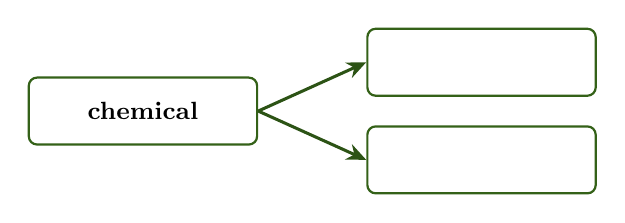
\begin{tikzpicture}
    \node[ebx] (p) at (0,0) {chemical};
    \node[ebx] (q) at (4.3,0.62) {};
    \node[ebx] (r) at (4.3,-0.62) {};
    \draw[earr] (p.east) -- (q.west);
    \draw[earr] (p.east) -- (r.west);
  \end{tikzpicture}
\end{minipage}
\end{minipage}

% -- E3 ---------------------------------------------------------------------
% The deck's bouncing ball with a new ball: a football from 2 m to 1.3 m.
% (b) is a decimal subtraction; (c) is the deck's "why not 2 m?".
\qhead[cbgreen]{E3}{The bouncing football}

\noindent\begin{minipage}{\textwidth}
Mr Bowen drops a football from \textbf{2 m}. It bounces up to \textbf{1.3 m}.
\fr{Mr Bowen l\^ache un ballon de foot de 2 m. Il rebondit jusqu'\`a 1.3 m.}

\vspace{4pt}
\noindent\textbf{(a)} Which store is the \textbf{biggest} at each moment? Use: \;
\eng{kinetic} \sep\ \eng{elastic potential} \sep\ \eng{gravitational potential}
\fr{(a) Quelle r\'eserve est la plus grande \`a chaque moment~?}

\vspace{4pt}
\noindent
\begin{tabularx}{\textwidth}{|L|C{6.6cm}|}
  \hline
  \textbf{Moment} & \textbf{Biggest store} \\ \hline
  in his hand, 2 m up \frin{dans sa main} \tall & {\color{cbteal}gravitational
    potential} \\ \hline
  just before it hits the floor \frin{juste avant le sol} \tall & \\ \hline
  squashed on the floor \frin{\'ecras\'e sur le sol} \tall & \\ \hline
  at the top of the bounce \frin{en haut du rebond} \tall & \\ \hline
\end{tabularx}
\end{minipage}

\vspace{6pt}
\begin{enumerate}[label=(\alph*), start=2, itemsep=\frl{5pt}{7pt}]
  \item How much lower than 2 m does it bounce?
        \fr{De combien rebondit-il plus bas que 2 m~?}
        \calcans
  \item \begin{minipage}[t]{\linewidth}
        Why does it not bounce back up to 2 m? Answer in a full sentence. \; Start:
        \eng{``At the bounce, some energy \ldots''}
        \fr{Pourquoi ne remonte-t-il pas jusqu'\`a 2 m~? R\'eponds par une phrase
        compl\`ete, en anglais.}
        \wlines{\frl{3}{3}}
        \end{minipage}
\end{enumerate}

% -- E4 ---------------------------------------------------------------------
% The write note: thermal energy moves from hotter to colder. (c) is the
% freezer vote, as Mr Bowen at the fridge.
\qhead[cbgreen]{E4}{Hotter to colder}

\noindent\begin{minipage}{\textwidth}
Mr Bowen's classroom is at $30\dC$. Does thermal energy move \textbf{into} each
drink, or \textbf{out of} it? Circle one.
\fr{La classe de Mr Bowen est \`a $30\dC$. L'\'energie thermique entre-t-elle dans
chaque boisson (\eng{into}) ou en sort-elle (\eng{out of})~? Entoure.}

\vspace{6pt}
{\renewcommand{\arraystretch}{1.6}%
\noindent\begin{tabular}{@{}l l l@{}}
  \textbf{(a)} & a hot coffee at $80\dC$ \frin{un caf\'e chaud} & \qquad
    \textbf{into} \quad\sep\quad \textbf{out of} \\
  \textbf{(b)} & a cold can of juice at $4\dC$ \frin{une canette froide} & \qquad
    \textbf{into} \quad\sep\quad \textbf{out of} \\
\end{tabular}}

\vspace{6pt}
\noindent\textbf{(c)} Mr Bowen opens the fridge. He says: \emph{``Close the door!
You are letting the cold out!''} Is he right? Explain. \; Start: \eng{``He is
\ldots, because thermal energy \ldots''}
\fr{(c) Mr Bowen ouvre le frigo. Il dit~: \fq{Ferme la porte~! Tu laisses sortir le
froid~!} A-t-il raison~? Explique, en anglais.}
\wlines{\frl{2}{3}}
\end{minipage}

% ===========================================================================
% SECTION F -- WHERE MATHS AND SCIENCE MEET
% ===========================================================================
\hwsection[cbblue]{Section F \textperiodcentered\ Maths and Science Together}

% -- F1 ---------------------------------------------------------------------
% THE KEYSTONE, and the packet's title. The two bulges are on a straight line
% through the Earth: 180 degrees apart. The Earth turns 15 degrees an hour,
% so 90 degrees (6 h) is high to low and 180 degrees (12 h) is high to high.
% (f) is the deck's "about 50 minutes later": 12 degrees x 4 minutes = 48.
\qhead[cbblue]{F1}{180\textdegree\ apart}

\noindent\begin{minipage}{\textwidth}
\noindent\begin{minipage}[c]{0.50\textwidth}\centering
  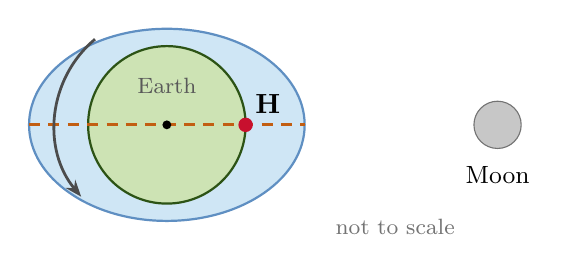
\begin{tikzpicture}
    \fill[seafill] (0,0) ellipse (1.75 and 1.22);
    \draw[cbblue!70, line width=0.8pt] (0,0) ellipse (1.75 and 1.22);
    \fill[landfill] (0,0) circle (1.0);
    \draw[cbgreen!60!black, line width=0.8pt] (0,0) circle (1.0);
    \draw[cborange, line width=1pt, dash pattern=on 4pt off 3pt] (-1.75,0) -- (1.75,0);
    \fill[black] (0,0) circle (1.6pt);
    \draw[black!70, line width=1pt, -{Stealth[length=6pt]}] (130:1.42) arc (130:220:1.42);
    \node[font=\footnotesize, text=black!65, align=center] at (0,0.5) {Earth};
    \fill[cbred] (1.0,0) circle (2.6pt);
    \node[font=\bfseries, anchor=south west] at (1.0,0.02) {H};
    \fill[black!22] (4.2,0) circle (0.3); \draw[black!55] (4.2,0) circle (0.3);
    \node[below=3pt, font=\small] at (4.2,-0.3) {Moon};
    \node[font=\footnotesize, text=black!55] at (2.9,-1.3) {not to scale};
  \end{tikzpicture}
\end{minipage}\hfill
\begin{minipage}[c]{0.47\textwidth}\raggedright
  The Earth seen from above the North Pole. The two bulges are on a
  \textbf{straight line} through the middle of the Earth. Mr Bowen's harbour
  \textbf{H} has high tide now.
  \fr{La Terre vue du dessus du p\^ole Nord. Les deux bosses d'eau sont sur une
  m\^eme ligne droite qui passe par le centre de la Terre. Le port H de Mr Bowen
  est \`a mar\'ee haute.}

  \vspace{4pt}
  The Earth \textbf{spins} once a day: \key{360\textdegree\ in 24 hours}.
  \fr{La Terre fait un tour sur elle-m\^eme par jour~: 360\textdegree\ en 24 heures.}
\end{minipage}
\end{minipage}

\vspace{6pt}
\noindent\textbf{(a)} How many degrees does the Earth turn in \textbf{1 hour}?
\fr{(a) De combien de degr\'es la Terre tourne-t-elle en 1 heure~?}
\calcans

\vspace{6pt}
\noindent\begin{minipage}{\textwidth}
\noindent\textbf{(b)} Complete the table.
\fr{(b) Compl\`ete le tableau.}

\vspace{3pt}
{\centering
\begin{tabular}{|l|*{5}{C{1.9cm}|}}
  \hline
  \textbf{Hours} & 1 & 3 & 6 & 12 & 24 \\ \hline
  \textbf{Degrees} \tall & {\color{cbteal}15\textdegree} & & & & 360\textdegree \\ \hline
\end{tabular}\par}
\end{minipage}

\vspace{8pt}
\begin{enumerate}[label=(\alph*), start=3, itemsep=\frl{6pt}{8pt}]
  \item After \textbf{6 hours}, H has turned through a \textbf{right angle}. Is H at
        high tide or low tide then? \hfill \blank[3.0cm]
        \fr{Apr\`es 6 heures, H a tourn\'e d'un angle droit. H est-il \`a mar\'ee haute
        ou \`a mar\'ee basse~?}
  \item After \textbf{12 hours}, H has turned $180\dg$. It is on the other side of
        the Earth. Is H at high tide or low tide? \hfill \blank[3.0cm]
        \fr{Apr\`es 12 heures, H a tourn\'e de $180\dg$~: il est de l'autre c\^ot\'e de
        la Terre. Mar\'ee haute ou mar\'ee basse~?}
  \item Complete: \ The two bulges are \blank[1.6cm]\textdegree\ apart. So H has a
        high tide every \blank[1.6cm] hours.
        \fr{Compl\`ete~: les deux bosses sont \`a \ldots\textdegree\ l'une de l'autre,
        donc H a une mar\'ee haute toutes les \ldots\ heures.}
  \item \begin{minipage}[t]{\linewidth}
        Every day the Moon moves on a little. So the Earth must turn about
        \textbf{12\textdegree\ more} to bring H back to the bulge. The Earth turns
        $1\dg$ every \textbf{4 minutes}. How many minutes later is high tide each
        day?
        \fr{Chaque jour, la Lune avance un peu. La Terre doit donc tourner d'environ
        12\textdegree\ de plus pour ramener H sous la bosse. La Terre tourne de
        $1\dg$ toutes les 4 minutes. Combien de minutes plus tard la mar\'ee haute
        arrive-t-elle chaque jour~?}
        \calcans
        \end{minipage}
\end{enumerate}

% -- F2 ---------------------------------------------------------------------
% The deck's LineThemUp model: a tidal range of 6 m with the Sun, the Moon and
% the Earth in a line, 2 m at right angles. In a line is 180 degrees at the
% Earth; at right angles the two lines are perpendicular.
\qhead[cbblue]{F2}{In a line, or at right angles?}

\noindent\begin{minipage}{\textwidth}
\noindent\begin{minipage}[b]{0.49\textwidth}\centering
  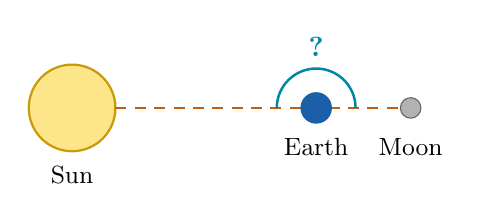
\begin{tikzpicture}
    \fill[sunfill] (0,0) circle (0.55); \draw[sunrim, line width=0.8pt] (0,0) circle (0.55);
    \node[font=\small] at (0,-0.85) {Sun};
    \draw[cborange, line width=1pt, dash pattern=on 4pt off 3pt] (0.55,0) -- (4.3,0);
    \fill[cbblue] (3.1,0) circle (0.2); \node[font=\small] at (3.1,-0.5) {Earth};
    \fill[black!30] (4.3,0) circle (0.13); \draw[black!60] (4.3,0) circle (0.13);
    \node[font=\small] at (4.3,-0.5) {Moon};
    \draw[cbteal, line width=0.9pt] (3.6,0) arc (0:180:0.5);
    \node[font=\bfseries, text=cbteal] at (3.1,0.78) {?};
  \end{tikzpicture}\par
  \textbf{(i)} full moon \frin{pleine lune}
\end{minipage}\hfill
\begin{minipage}[b]{0.49\textwidth}\centering
  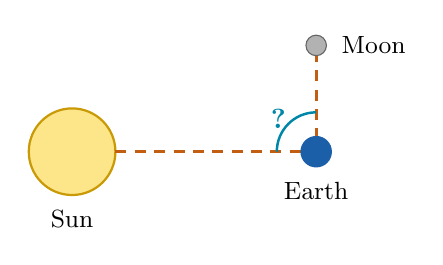
\begin{tikzpicture}
    \fill[sunfill] (0,0) circle (0.55); \draw[sunrim, line width=0.8pt] (0,0) circle (0.55);
    \node[font=\small] at (0,-0.85) {Sun};
    \draw[cborange, line width=1pt, dash pattern=on 4pt off 3pt] (0.55,0) -- (3.1,0)
      -- (3.1,1.35);
    \fill[cbblue] (3.1,0) circle (0.2); \node[font=\small] at (3.1,-0.5) {Earth};
    \fill[black!30] (3.1,1.35) circle (0.13); \draw[black!60] (3.1,1.35) circle (0.13);
    \node[font=\small, anchor=west] at (3.3,1.35) {Moon};
    \draw[cbteal, line width=0.9pt] (3.1,0.5) arc (90:180:0.5);
    \node[font=\bfseries, text=cbteal] at (2.62,0.42) {?};
  \end{tikzpicture}\par
  \textbf{(ii)} half moon \frin{demi-lune}
\end{minipage}

\vspace{2pt}
{\centering\footnotesize\color{black!55} seen from above the North Pole, not to
scale\par}

\vspace{6pt}
\noindent\textbf{(a)} Write the angle \textbf{?} at the Earth, between the line to the
Sun and the line to the Moon.
\par\nobreak\vspace{4pt}\noindent\hspace*{1.6em}\textbf{(i)} \blank[2.2cm] \qquad
\textbf{(ii)} \blank[2.2cm]
\fr{(a) \'Ecris l'angle \textbf{?} au niveau de la Terre, entre la ligne vers le
Soleil et la ligne vers la Lune.}

\vspace{6pt}
\noindent\textbf{(b)} In \textbf{(ii)}, the two lines are \quad \textbf{parallel}
\quad\sep\quad \textbf{perpendicular}. \ Circle one.
\fr{(b) Dans (ii), les deux lignes sont parall\`eles ou perpendiculaires~? Entoure.}
\end{minipage}

\vspace{6pt}
\begin{enumerate}[label=(\alph*), start=3, itemsep=\frl{6pt}{8pt}]
  \item In the lesson's model, the tidal range at Mr Bowen's harbour was
        \textbf{6 m} in one picture and \textbf{2 m} in the other. Which picture had
        the 6 m tides? \hfill \blank[1.8cm]
        \fr{Dans le mod\`ele de la le\c{c}on, le marnage du port de Mr Bowen \'etait de
        6 m dans un dessin et de 2 m dans l'autre. Quel dessin avait les mar\'ees de
        6 m~?}
  \item How much \textbf{bigger} is the 6 m range? \ How many \textbf{times as big}?
        \fr{De combien le marnage de 6 m est-il plus grand~? Combien de fois plus
        grand~?}
        \par\nobreak\vspace{\frl{4pt}{6pt}}\noindent\hspace*{1.6em}%
        \textbf{Bigger by:} \blank[4.6cm] \hfill \textbf{Times as big:} \blank[4.0cm]
  \item \begin{minipage}[t]{\linewidth}
        Why are the tides biggest when the Sun, the Moon and the Earth are in a
        line? \; Start: \eng{``When they are in a line, the Sun's tidal force
        \ldots''}
        \fr{Pourquoi les mar\'ees sont-elles les plus grandes quand le Soleil, la Lune
        et la Terre sont align\'es~? R\'eponds en anglais.}
        \wlines{\frl{2}{3}}
        \end{minipage}
\end{enumerate}

% -- F3 ---------------------------------------------------------------------
% A pizza whose angles are its joules: 3 600 000 J over 360 degrees is
% 10 000 J a degree. (b) is 5.2's pizza with new numbers: vertically opposite,
% then a straight line. (d) is 3.5's kettle-to-floors comparison.
\qhead[cbblue]{F3}{A slice of energy}

\noindent\begin{minipage}{\textwidth}
Food has a \textbf{chemical} store. Mr Bowen's pizza stores \key{3\,600\,000 J}.
So every \key{1\textdegree} of pizza stores \key{10\,000 J}.
\fr{La nourriture a une r\'eserve chimique. La pizza de Mr Bowen stocke 3\,600\,000 J.
Donc chaque degr\'e (1\textdegree) de pizza stocke 10\,000 J.}

\vspace{4pt}
\begin{enumerate}[label=(\alph*), itemsep=\frl{6pt}{8pt}]
  \item He cuts it into \textbf{8 equal slices}. What angle is one slice? How many
        joules does one slice store?
        \fr{Il la coupe en 8 parts \'egales. Quel est l'angle d'une part~? Combien de
        joules une part stocke-t-elle~?}
        \par\nobreak\vspace{\frl{4pt}{6pt}}\noindent\hspace*{1.6em}%
        \textbf{Angle:} \blank[4.2cm] \hfill \textbf{Joules:} \blank[5.0cm]
\end{enumerate}
\end{minipage}

\vspace{6pt}
\noindent\begin{minipage}{\textwidth}
\noindent\begin{minipage}[c]{0.34\textwidth}\centering
  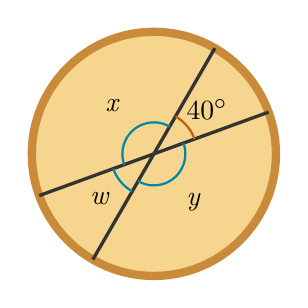
\begin{tikzpicture}
    \coordinate (O) at (0,0);
    \coordinate (P1) at (20:1.55); \coordinate (P2) at (60:1.55);
    \coordinate (P3) at (200:1.55); \coordinate (P4) at (240:1.55);
    \fill[pizzafill] (O) circle (1.55);
    \draw[crust, line width=3pt] (O) circle (1.55);
    \draw[black!80, line width=1.2pt] (P1) -- (P3);
    \draw[black!80, line width=1.2pt] (P2) -- (P4);
    \pic[ang, "$40\dg$", angle radius=0.55cm, angle eccentricity=1.6] {angle = P1--O--P2};
    \pic[let, "$x$", angle radius=0.4cm, angle eccentricity=2.0] {angle = P2--O--P3};
    \pic[let, "$w$", angle radius=0.55cm, angle eccentricity=1.6] {angle = P3--O--P4};
    \pic[let, "$y$", angle radius=0.4cm, angle eccentricity=2.0] {angle = P4--O--P1};
  \end{tikzpicture}
\end{minipage}\hfill
\begin{minipage}[c]{0.63\textwidth}\raggedright
  \textbf{(b)} The next pizza: he makes \textbf{two straight cuts}. One slice is
  $40\dg$. Find $w$, $x$ and $y$. Give a reason for each.
  \fr{(b) Pizza suivante~: il fait deux coupes droites. Une part fait $40\dg$.
  Trouve $w$, $x$ et $y$, avec une raison pour chacun (en anglais).}

  \vspace{4pt}
  {\renewcommand{\arraystretch}{\frl{1.75}{2.0}}%
  \begin{tabular}{@{}l@{\ }l@{\ \ }l@{}}
    $w =$ & \blank[1.3cm] & because \blank[5.2cm] \\
    $x =$ & \blank[1.3cm] & because \blank[5.2cm] \\
    $y =$ & \blank[1.3cm] & because \blank[5.2cm] \\
  \end{tabular}}
\end{minipage}
\end{minipage}

\vspace{6pt}
\begin{enumerate}[label=(\alph*), start=3, itemsep=\frl{6pt}{8pt}]
  \item He eats the \textbf{two biggest} slices. How many degrees of pizza is that?
        How many joules?
        \fr{Il mange les deux plus grosses parts. Cela fait combien de degr\'es de
        pizza~? Combien de joules~?}
        \par\nobreak\vspace{\frl{4pt}{6pt}}\noindent\hspace*{1.6em}%
        \textbf{Degrees:} \blank[4.0cm] \hfill \textbf{Joules:} \blank[5.0cm]
  \item One floor of stairs uses \textbf{2\,000 J}. How many floors could he climb
        with the energy in those two slices? \ (Landmark 81 has 81 floors.)
        \fr{Un \'etage d'escalier demande 2\,000 J. Combien d'\'etages pourrait-il
        monter avec l'\'energie de ces deux parts~? (Le Landmark 81 a 81 \'etages.)}
        \calcans
\end{enumerate}

% -- F4 ---------------------------------------------------------------------
% Angles round a point (5.1), then two energy-change diagrams (3.6) that are
% each other backwards: the turbine is kinetic to electrical (3.6's wind farm
% at Bac Lieu), the fan electrical to kinetic, with sound as well.
\qhead[cbblue]{F4}{The wind turbine and the fan}

\noindent\begin{minipage}{\textwidth}
\noindent\begin{minipage}[b]{0.49\textwidth}\centering
  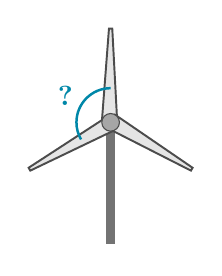
\begin{tikzpicture}[scale=0.7]
    \draw[black!55, line width=3pt] (0,-0.1) -- (0,-2.2);
    \foreach \a in {90, 210, 330}
      \filldraw[fill=black!10, draw=black!70, line width=0.7pt]
        ($(\a-90:0.12)$) -- ($(\a:1.7)+(\a-90:0.03)$) -- ($(\a:1.7)+(\a+90:0.03)$)
        -- ($(\a+90:0.16)$) -- cycle;
    \filldraw[fill=black!35, draw=black!70] (0,0) circle (0.16);
    \draw[cbteal, line width=0.9pt] (90:0.62) arc (90:210:0.62);
    \node[font=\bfseries, text=cbteal] at (150:0.95) {?};
  \end{tikzpicture}\par
  a \textbf{wind turbine}: 3 blades \frin{une \'eolienne}
\end{minipage}\hfill
\begin{minipage}[b]{0.49\textwidth}\centering
  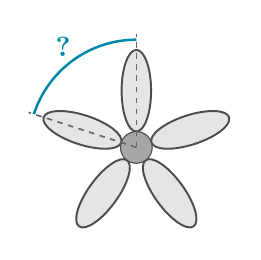
\begin{tikzpicture}[scale=0.72]
    \foreach \a in {90, 162, 234, 306, 18}
      \filldraw[fill=black!10, draw=black!70, line width=0.7pt, rotate=\a]
        (1.0,0) ellipse (0.72 and 0.26);
    \filldraw[fill=black!35, draw=black!70] (0,0) circle (0.28);
    \draw[black!60, line width=0.6pt, dash pattern=on 2pt off 2pt] (0,0) -- (90:2.0);
    \draw[black!60, line width=0.6pt, dash pattern=on 2pt off 2pt] (0,0) -- (162:2.0);
    \draw[cbteal, line width=0.9pt] (90:1.9) arc (90:162:1.9);
    \node[font=\bfseries, text=cbteal] at (126:2.2) {?};
  \end{tikzpicture}\par
  a \textbf{ceiling fan}: 5 blades \frin{un ventilateur de plafond}
\end{minipage}

\vspace{6pt}
\noindent\textbf{(a)} The blades are \textbf{equally} spaced. Work out each angle
\textbf{?}
\fr{(a) Les pales sont \'egalement espac\'ees. Calcule chaque angle \textbf{?}}

\vspace{2pt}
\noindent\hspace*{1.6em}\textbf{Turbine:} \blank[4.6cm] \hfill \textbf{Fan:}
\blank[4.6cm]
\end{minipage}

\vspace{8pt}
\noindent\begin{minipage}{\textwidth}
\noindent\textbf{(b)} Fill in the energy-change diagrams. Use: \; \eng{kinetic}
\sep\ \eng{electrical} \sep\ \eng{sound}
\fr{(b) Compl\`ete les sch\'emas de transformation.}

\vspace{4pt}
\noindent\begin{minipage}[t]{0.49\textwidth}
  \textbf{Turbine} \frin{l'\'eolienne}\par\vspace{4pt}
  
\begin{tikzpicture}
    \node[ebx] (p) at (0,0) {}; \node[ebx] (q) at (4.3,0) {};
    \draw[earr] (p) -- (q);
  \end{tikzpicture}
\end{minipage}\hfill
\begin{minipage}[t]{0.49\textwidth}
  \textbf{Fan} \frin{le ventilateur}\par\vspace{4pt}
  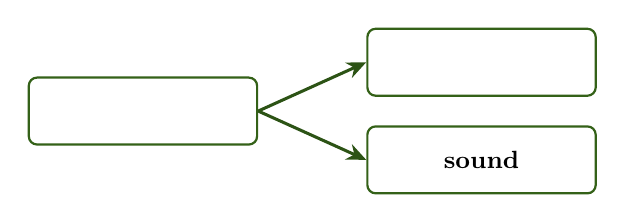
\begin{tikzpicture}
    \node[ebx] (p) at (0,0) {};
    \node[ebx] (q) at (4.3,0.62) {}; \node[ebx] (r) at (4.3,-0.62) {sound};
    \draw[earr] (p.east) -- (q.west); \draw[earr] (p.east) -- (r.west);
  \end{tikzpicture}
\end{minipage}

\vspace{6pt}
\noindent\textbf{(c)} What do you notice about the two diagrams? Answer in a full
sentence. \; Start: \eng{``The fan's energy change is \ldots''}
\fr{(c) Que remarques-tu sur les deux sch\'emas~? R\'eponds par une phrase compl\`ete,
en anglais.}
\wlines{\frl{2}{3}}
\end{minipage}

% -- F5 ---------------------------------------------------------------------
% The writing. Mr Bowen is wrong (one bulge, one high tide); the reply has to
% use the maths of F1 to put him right.
\qhead[cbblue]{F5}{Explain it with maths}

\noindent\begin{minipage}{\textwidth}
Mr Bowen says: \emph{``The Moon is on one side of the Earth. So there is only
\textbf{one} high tide a day.''} \ Write him a reply in English: 4 or 5 sentences.
\fr{Mr Bowen dit~: \fq{La Lune est d'un seul c\^ot\'e de la Terre. Donc il n'y a
qu'une seule mar\'ee haute par jour.} \'Ecris-lui une r\'eponse en anglais, en 4 ou 5
phrases.}

\begin{yourturn}[Your reply must have: tick each one]
  \renewcommand{\arraystretch}{1.35}%
  \begin{tabularx}{\linewidth}{@{}p{0.75cm}L p{0.75cm}L p{0.75cm}L@{}}
    \tickbox & \textbf{tidal force} & \tickbox & \textbf{two bulges} &
      \tickbox & \textbf{180\textdegree} apart \\
    \tickbox & the Earth \textbf{spins} & \tickbox & \textbf{12 hours} & \tickbox &
      full sentences \\
  \end{tabularx}
  \fr{La force de mar\'ee, les deux bosses, 180\textdegree\ d'\'ecart, la Terre qui
  tourne, 12 heures, des phrases compl\`etes.}
\end{yourturn}
\wlines{\frl{6}{6}}
\end{minipage}

% ===========================================================================
% ANSWER KEY -- TEACHER COPY ONLY
% ===========================================================================
\ifkey
\clearpage

\hwsection[cbred]{Answer Key --- Teacher Copy}

\linespread{1.0}\selectfont
\setlist[enumerate]{itemsep=2pt, topsep=3pt, leftmargin=*}
\setlist[itemize]{itemsep=2pt, topsep=3pt, leftmargin=*}

\qhead[cbred]{A1}{Two steps}
\noindent (b) $180\dg - 72\dg = \mathbf{108\dg}$ \quad (c) $125 + 80 + 95 = 300$, \
$360 - 300 = \mathbf{60\dg}$ \quad (d) $90 + 132 = 222$, \ $360 - 222 =
\mathbf{138\dg}$ \\
(e) $64 + 105 + 118 = 287$, \ $360 - 287 = \mathbf{73\dg}$ \quad (f) $q =
\mathbf{58\dg}$ (opposite); \ $360 - 58 - 58 = 244$, \ $p = r = 244 \div 2 =
\mathbf{122\dg}$

\smallskip
\noindent{\small Every diagram is drawn accurately, so a protractor checks any answer
--- worth saying to a student who is stuck. \\
(b) has one known angle, so step 1 is just $72\dg$; expect $252\dg$ ($180 + 72$) from
anyone who adds when they should subtract. \\
(c) and (d) are \emph{round a point}: expect $180 - 300$ (impossible) or $180 - 222$
from a student who uses 180 for everything. The fix is the first question of the
two steps: \emph{180 or 360?} \\
(d) has a small square: a right angle, $90\dg$, not written as a number. Expect
$228\dg$ ($360 - 132$) from anyone who skipped it. \\
(f) is the deck's parallelogram with new numbers; $p = 122$ and $q = 122$ means the
student paired the wrong corners (opposite = across the shape, not next to it).}

\qhead[cbred]{A2}{From English to a calculation}
\noindent (a) $63 + 116 = 179\dg$: \textbf{no}, a straight line is $180\dg$ \quad
(b) $180 - 64 = 116\dg$ \\
(c) $360 - (90 + 90 + 47) = 360 - 227 = 133\dg$ \quad (d) $360 - 120 = 240$, \ $240
\div 3 = 80\dg$ \quad (e) $1080 \div 360 = 3$ full turns

\smallskip
\noindent{\small \textbf{Mark the calculation, not the answer.} \\
(a) is the deck's vote (57 + 121 = 178) with new numbers. It looks straight; the
point is that you \emph{add}, you do not look. ``Yes'' with no calculation is the
error the vote was for. \\
(b) ``The sum of two angles is 180'' is a straight line without the picture. A
student who writes $180 + 64$ read \emph{sum} and added the numbers they could see:
have them read the word-help line aloud. \\
(d) is two steps and the second is a division: expect $240\dg$, which is the three
angles together. \\
(e) runs the deck's chair backwards (there: $2.5 \times 360 = 900$). Expect $1080
\times 360$ from a student who sees two numbers and multiplies. He is facing the
board again; the lesson has not moved.}

\qhead[cbred]{A3}{Now you write the question}
\noindent{\small Check, in order: a quadrilateral (or a four-sided real thing called
one); three angles $70\dg$, $110\dg$, $95\dg$; it asks for the fourth; it ends in a
question mark; it uses full sentences. $70 + 110 + 95 + 85 = 360$. \\
Model: \emph{``Mr Bowen's garden is a quadrilateral. Three of its angles are
70\textdegree, 110\textdegree\ and 95\textdegree. What size is the fourth angle?''} \\
The usual failure is a question whose answer is not $85\dg$ --- e.g. one that gives
all four angles, or asks for their sum. A question about a triangle has the wrong
total; ask the student what $360\dg$ is for.}

\qhead[cbred]{B1}{Find the angle. Give a reason.}
\noindent $b = 43\dg$ because angles on a straight line add up to $180\dg$ ($180 -
137$). \\
$c = 62\dg$ because corresponding angles are equal. \\
$d = 74\dg$ because alternate angles are equal. \\
$e = 106\dg$ because angles on a straight line add up to $180\dg$ ($180 - 74$). \\
(iv) \textbf{C}, because there are no arrows, so we do not know that the lines are
parallel.

\smallskip
\noindent{\small Accept the reason in the student's own words if the fact is right
(``they make a Z'' is fine for $d$). A right number with no reason is half done:
the reason is the 5.2 skill. \\
$b = 137\dg$ means the student called every angle at an X ``vertically opposite''.
$b$ is \emph{next to} $137\dg$, not opposite it. \\
(iv) The lines look parallel and $68\dg$ is tempting; \textbf{A} is the error the
deck's slide 21 was for. \textbf{B} ($112\dg$) is worse: it is a guess with a
subtraction in it.}

\qhead[cbred]{B2}{Mr Bowen's homework}
\noindent (a) \textbf{wrong}: $b = 70\dg$ because \emph{vertically opposite} angles
are equal. \\
(b) \textbf{wrong}: $e = 70\dg$ because they are \emph{corresponding} angles. \\
(c) \textbf{wrong}: $a = 110\dg$ because angles on a straight line add up to
$180\dg$. \\
(d) \textbf{right} ($c = 110\dg$, and $c$ and $d$ make a Z).

\smallskip
\noindent{\small (a) and (b) have the right \emph{number} and the wrong \emph{name}.
A student who writes ``right'' for them is checking the arithmetic, not the reason:
point at the word ``completely''. \\
(c) is the trap from the other side: $a$ is \emph{next to} the $70\dg$, so it is
$110\dg$. A correction that keeps $70\dg$ and changes only the reason has missed
it. \\
(d) needs $c$ first, and $c$'s size is not given. Students who mark it wrong because
``we don't know $c$'' should find it ($180 - 70$) and look again.}

\qhead[cbred]{C1}{A day at the harbour}
\noindent (a) 2 \quad (b) 6 hours \quad (c) $5.7 - 1.3 = 4.4$ m \\
(d) \emph{No, because the Moon moves on a little every day, so high tide is about 50
minutes later (about 3:50 a.m.).}

\smallskip
\noindent{\small (b) Expect 12 (high to \emph{high}). \\
(d) Accept any answer that says ``later'' and gives the Moon moving as the reason;
the 50 minutes is a bonus. ``The Earth moves'' alone is not the reason --- it moves
every day. \\
The book's Question 6 (average depth and range: not 7.0 m) is Extra Homework 11's
X3, so it is not repeated here.}

\qhead[cbred]{C2}{Two high tides at the same time}
\noindent (a) A \textbf{H} \sep B \textbf{L} \sep C \textbf{H} \sep D \textbf{L} \\
(b) \emph{The near side is pulled the most. The far side is pulled the least, so it
is left behind, and the water makes a bulge there too.}

\smallskip
\noindent{\small (a) C written as L is the deck's vote all over again (``one bulge'').
If it is common, act out the three students again: 3 steps, 2 steps, 1 step. The
middle is the Earth; the 1-step student is the far bulge, left behind. Section F1 and
F5 lean on this.}

\qhead[cbred]{C3}{The Sun, and the land}
\noindent (a) \emph{The Sun is much further away (390 times), so it stretches the
Earth less.} \\
(b) \emph{We do not feel it because everything goes up and down together: the
ground, the buildings and us.}

\smallskip
\noindent{\small (a) ``The Sun is far away, so its gravity is weak'' contradicts the
question (it says the Sun's pull is stronger). The word to look for is
\emph{stretch}: tides come from the stretch, not the pull.}

\qhead[cbred]{D1}{Mr Bowen's afternoon in joules}
\noindent (a) $4 \times 2\,000 = 8\,000$ J \quad (b) $45 \times 200 = 9\,000$ J \quad
(c) $0.5 \times 400\,000 = 200\,000$ J \\
(d) $200\,000 \div 8\,000 = 25$ times

\smallskip
\noindent{\small (c) is half of 400\,000 (4.5's quick way: $\times 0.5$ is half).
Expect 2\,000\,000 or 20\,000 from a student who moved the point instead of halving.
\\
(d) is ``how many times'': divide. $200\,000 - 8\,000 = 192\,000$ is the HW 10 trap
(\emph{how much more} against \emph{how many times as much}) again.}

\qhead[cbred]{D2}{Mr Bowen's bike ride at night}
\noindent 2 gravitational potential, store \sep 3 chemical, store \sep 4 light,
transfer \sep 5 electrical, transfer \sep 6 sound, transfer \sep 7 thermal, store
(accept transfer) \sep 8 elastic potential, store

\smallskip
\noindent{\small Row 3 is food, and food is chemical: ``kinetic'' (because Mr Bowen is
riding) has read the wrong part of the clue. Row 7 is thermal either way: the hot
brakes store it, and they heat the air. Accept both.}

\qhead[cbred]{D3}{Which stores last?}
\noindent tea \textbf{N} \sep rice \textbf{Y} \sep spinning top \textbf{N} \sep rock
\textbf{Y}

\smallskip
\noindent{\small The write note: chemical and gravitational potential last; thermal
and kinetic do not. A student who writes Y for the tea is thinking of the drink,
not its heat: the drink lasts, its thermal store goes into the room in an hour
(E4 asks which way).}

\qhead[cbred]{E1}{An event or a process?}
\noindent plate \textbf{event} \sep Sun \textbf{process} \sep balloon \textbf{event}
\sep candle \textbf{process} \sep firework \textbf{event} \sep fridge
\textbf{process}

\qhead[cbred]{E2}{Energy-change diagrams}
\noindent (a) thermal \sep (b) chemical \sep (c) gravitational potential \sep (d)
kinetic $\to$ thermal \sep (e) light and thermal (either order)

\smallskip
\noindent{\small (b) is the deck's vote: \emph{electrical} in the empty box means
the student thinks a battery stores electricity. It stores \emph{chemical} energy. \\
(a) accept ``thermal'' or ``thermal and light'' (a glowing toaster). \\
(d) is the deck's ``rub your hands'': kinetic \emph{to} thermal.}

\qhead[cbred]{E3}{The bouncing football}
\noindent (a) kinetic \sep elastic potential \sep gravitational potential \\
(b) $2 - 1.3 = 0.7$ m \\
(c) \emph{At the bounce, some energy changed to sound and heat, so it cannot lift the
ball back up to 2 m.}

\smallskip
\noindent{\small (b) Expect $1.1$ ($2 - 1.3$ worked as $3 - 2$, or 13 $-$ 2) from a
student who does not write $2 = 2.0$. \\
(c) ``Gravity pulls it down'' is not the reason --- gravity pulled it down on the
way \emph{down} too. ``The energy is lost'' is half: say where it went.}

\qhead[cbred]{E4}{Hotter to colder}
\noindent (a) out of \sep (b) into \\
(c) \emph{He is wrong, because thermal energy moves from hotter things to colder
things. Heat from the warm room goes into the fridge; cold does not come out.}

\smallskip
\noindent{\small (c) is the freezer vote in 3.6 (``does cold go in, or heat come
out?''). ``He is right because the food gets warm'' gets the result right and the
direction wrong.}

\qhead[cbred]{F1}{180\textdegree\ apart}
\noindent (a) $360 \div 24 = 15\dg$ \quad (b) 3 h $45\dg$ \sep 6 h $90\dg$ \sep 12 h
$180\dg$ \\
(c) low tide \quad (d) high tide \quad (e) $180\dg$; every 12 hours \\
(f) $12 \times 4 = 48$ minutes: \emph{about 50 minutes later}, like the lesson.

\smallskip
\noindent{\small \textbf{This is the question the packet is named for.} The two
bulges are on one straight line through the Earth, so they are $180\dg$ apart, and
the Earth needs 12 hours to turn $180\dg$. That is why high tide comes every 12
hours and low tide 6 hours (a right angle) after it. \\
(d) ``Low'' means the student thinks of one bulge (C2 again). \\
(f) The 12 is $360 \div 29$: the Moon goes round in about 29 days. The 4 minutes is
$24 \times 60 = 1\,440$ minutes $\div\ 360$. Both are worth asking the strongest
students to check. 48 is the deck's ``about 50'' ($24$ hours $\div\ 29$).}

\qhead[cbred]{F2}{In a line, or at right angles?}
\noindent (a) (i) $180\dg$ \sep (ii) $90\dg$ \quad (b) perpendicular \\
(c) (i) \quad (d) $6 - 2 = 4$ m bigger; $6 \div 2 = 3$ times as big \\
(e) \emph{When they are in a line, the Sun's tidal force pulls the oceans the same
way as the Moon's, so they add up and the bulges are bigger.}

\smallskip
\noindent{\small The 6 m and 2 m are the deck's \emph{Line Them Up} model (Mr Bowen's
harbour). New moon is in a line too: the angle at the Earth is $0\dg$ there, which
is worth raising with anyone who asks. \\
(d) is the HW 10 pair again: \emph{how much bigger} subtracts, \emph{how many times}
divides.}

\qhead[cbred]{F3}{A slice of energy}
\noindent (a) $360 \div 8 = 45\dg$; \ $45 \times 10\,000 = 450\,000$ J \\
(b) $w = 40\dg$ because vertically opposite angles are equal; \ $x = 140\dg$ because
angles on a straight line add up to $180\dg$; \ $y = 140\dg$ (vertically opposite
$x$, or a straight line) \\
(c) $140 + 140 = 280\dg$; \ $280 \times 10\,000 = 2\,800\,000$ J \\
(d) $2\,800\,000 \div 2\,000 = 1\,400$ floors

\smallskip
\noindent{\small (a) One slice (450\,000 J) is more than boiling a litre of water
(400\,000 J): worth saying aloud. \\
(b) is the 5.2 deck's pizza with new numbers. \\
(d) is 3.5's kettle-to-stairs comparison; 1\,400 floors is 17 Landmark 81s. A real
body turns most of that energy into heat, not stairs --- 3.7 will say so. He takes
the lift. \\
Expect 28\,000\,000 or 280\,000 in (c) from a student who loses count of zeros:
$\times 10\,000$ is four zeros.}

\qhead[cbred]{F4}{The wind turbine and the fan}
\noindent (a) turbine $360 \div 3 = 120\dg$ \sep fan $360 \div 5 = 72\dg$ \\
(b) turbine: kinetic $\to$ electrical \sep fan: electrical $\to$ kinetic (and sound)
\\
(c) \emph{The fan's energy change is the turbine's backwards: the turbine changes
kinetic energy to electrical energy, and the fan changes electrical energy to
kinetic energy.}

\smallskip
\noindent{\small The turbine is the 3.6 deck's Bac Lieu wind farm. A student who
draws ``wind'' in the turbine's first box has the idea; ask what kind of energy
moving air has.}

\qhead[cbred]{F5}{Explain it with maths}
\noindent{\small Check the six ticks. A model reply: \emph{``There are two high tides
a day, not one. The Moon's tidal force pulls the oceans into two bulges, one on each
side of the Earth. The bulges are on a straight line, 180\textdegree\ apart. The Earth
spins 15\textdegree\ every hour, so it takes 12 hours to turn 180\textdegree\ from one
bulge to the other. So every harbour has a high tide every 12 hours.''} \\
The thinking to look for is the \emph{why} of the far bulge (the stretch, from C2)
joined to the \emph{when} (12 hours, from F1). A reply that only says ``the Earth
spins'' explains one high tide a day, which is Mr Bowen's mistake.}

\fi

\end{document}
